% Copyright (C) 2010,2011,2012,2013,2014,2015,2016 The ESPResSo project
% Copyright (C) 2002,2003,2004,2005,2006,2007,2008,2009,2010 
%   Max-Planck-Institute for Polymer Research, Theory Group
%  
% This file is part of ESPResSo.
%   
% ESPResSo is free software: you can redistribute it and/or modify it
% under the terms of the GNU General Public License as published by the
% Free Software Foundation, either version 3 of the License, or (at your
% option) any later version.
%  
% ESPResSo is distributed in the hope that it will be useful, but
% WITHOUT ANY WARRANTY; without even the implied warranty of
% MERCHANTABILITY or FITNESS FOR A PARTICULAR PURPOSE.  See the GNU
% General Public License for more details.
%  
% You should have received a copy of the GNU General Public License
% along with this program.  If not, see <http://www.gnu.org/licenses/>.
%
\documentclass[
a4paper,                        % paper size
11pt,                           % font size
twoside,                        % two sided
footsepline,                    % add a line to separate the footer
headsepline,                    % add a line to separate the header
headexclude,                    % header does not belong to the text
footexclude,                    % footer does not belong to the text
pagesize,                       % set the pagesize in a DVI document
]{scrartcl}

% Copyright (C) 2010,2011,2012 The ESPResSo project
% Copyright (C) 2002,2003,2004,2005,2006,2007,2008,2009,2010
%  Max-Planck-Institute for Polymer Research, Theory Group
%  
% This file is part of ESPResSo.
%   
% ESPResSo is free software: you can redistribute it and/or modify it
% under the terms of the GNU General Public License as published by the
% Free Software Foundation, either version 3 of the License, or (at your
% option) any later version.
%  
% ESPResSo is distributed in the hope that it will be useful, but
% WITHOUT ANY WARRANTY; without even the implied warranty of
% MERCHANTABILITY or FITNESS FOR A PARTICULAR PURPOSE.  See the GNU
% General Public License for more details.
%  
% You should have received a copy of the GNU General Public License
% along with this program.  If not, see <http://www.gnu.org/licenses/>.
%
\usepackage[draft]{varioref}    % defines \vref
\usepackage{hyperref}           % automatically creates links when
                                % using pdflatex, defines \url
\usepackage{ifpdf}              % defines \ifpdf
\usepackage{graphicx}           % handles graphics
\usepackage{color}              % use colors

\usepackage{amsmath}

\usepackage{verbatim}           % required for \verbatim and \endverbatim
\usepackage{fancyvrb}
\usepackage{calc}               % compute length
\usepackage{ifthen}             % provide ifthen
\usepackage{xspace}
\usepackage{units}
\usepackage[numbers]{natbib}

% For building the distribution docs, disable todo boxes.
%\usepackage[disable]{todonotes}
\usepackage{todonotes}

\newcommand{\es}{\mbox{\textsf{ESPResSo}}\xspace}
\newcommand{\ie}{\textit{i.e.}\xspace}
\newcommand{\eg}{\textit{e.g.}\xspace}
\newcommand{\etal}{\textit{et al.}\xspace}

\newcommand{\codebox}[1]%
{\texttt{#1}}

\DefineVerbatimEnvironment{code}{Verbatim}%
{commandchars=\\\{\}}
\makeatletter
\newenvironment{tclcode}
{%
  \addtolength{\linewidth}{-2em}% set the line length
  \@minipagetrue%%%DPC%%%
  \@tempswatrue%%%DPC%%%
  \hsize=\linewidth%
  \setbox0=\vbox\bgroup\verbatim
}{\endverbatim
  \unskip\setbox0=\lastbox%%%DPC%%%
  \egroup
  \par%
  \noindent\hspace{1em}%
  \codebox{\box0}%
  \par\noindent%
}
\makeatother

% \newcommand{\todo}[1]{
%   \marginpar{%
%     \setlength{\fboxrule}{1pt}
%     \fcolorbox{red}{yellow}{%
%       \parbox{\marginparwidth-2\fboxrule-2\fboxsep}{%
%         \bf\raggedright\scriptsize #1%
%       }%
%     }%
%   }%
% }

\makeatletter
\renewcommand{\minisec}[1]{\@afterindentfalse \vskip 1.5ex
  {\parindent \z@
    \raggedsection\normalfont\sffamily\itshape\nobreak#1\par\nobreak}%
  \@afterheading}
\makeatother

\newcommand{\esptitlehead}{
  \titlehead{
    \begin{center}
      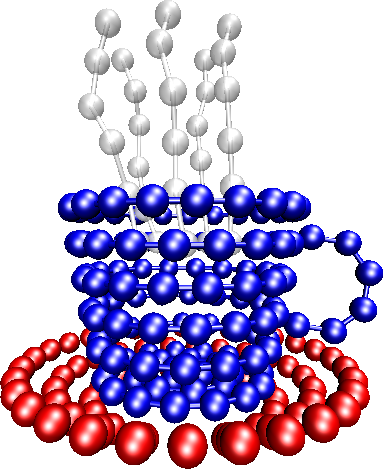
\includegraphics[width=5cm]{logo/transparentbg}
    \end{center}
  }
}


\lstset{language=Python} 

\begin{document}
\esptitlehead
\title{Tutorial 2: A simple charged system%
\ifdefined\esversion%
\thanks{For \es \esversion}%
\fi%
}

\maketitle
\tableofcontents

\section{Introduction}

This tutorial introduces some of the basic features of \es\ for charged systems
by constructing a simulation script for a simple salt crystal. We assume that
the reader is familiar with the basic concepts of Python and MD simulations. The
code pieces can be copied step by step into a python script file, which then can
be run using \verb|pypresso <file>| from the \es build directory.

\section{Basic setup}

Our script starts with python imports and setting up the system.
Most conveniently, one would like to specify the density and the number of
particles of the system as parameters:

\begin{lstlisting}
import espressomd
from espressomd import thermostat
from espressomd import electrostatics
from espressomd import code_info
from espressomd import integrate
import numpy

# Setup system 
n_part = 200
density = 0.7
box_l = (n_part / density)**(1. / 3.)

system = espressomd.System()
system.box_l = [box_l, box_l, box_l]
system.periodicity = [1, 1, 1]
system.time_step = 0.01
system.skin = 0.3
\end{lstlisting}

The box length is calculated from the number of particles and the system
density. This allows to change the parameters later easily, e.~g.\ to simulate a
bigger system. The parameters of the simulation engine are modified by changing the
espressomd.System() properties. We define a cubic simulation box of size 
\verb|box_l| and periodic boundary conditions in all spatial dimensions. 
We now fill this simulation box with particles:

\begin{lstlisting}
# Place particles
q = 1.
ptype = 0
for i in xrange(n_part):
    q *= -1
    ptype = 1 - ptype
    system.part.add(id=i, 
                    type=ptype, 
                    pos=numpy.random.random(3) * system.box_l, 
                    q=q)
\end{lstlisting}

This loop adds \verb|n_part| particles at random positions. The \verb|part|
command is used to specify particle properties, unique integer id, position, charge \verb|q| and
type. In \es\ the particle type is just an integer number which allows to group
particles. We alternate between creating positive charges of type 0 and negative
charges of type 1. 

Now we define the ensemble that we will be simulating. This is done
using the \verb|thermostat| class. 

\begin{lstlisting}
# Thermostat
temp = 1.
gamma = 1.
thermostat.Thermostat().set_langevin(kT=temp, gamma=gamma)
\end{lstlisting}

This switches on the Langevin thermostat for the NVT ensemble, with
temperature \verb|temp| and friction coefficient \verb|gamma|. 
Before we can really start the simulation, we have to specify the
interactions between our particles. We use a simple, purely repulsive
Lennard-Jones interaction to model a hard core repulsion: 

\begin{lstlisting}
# Lennard-Jones interactions
lj_sig = 1.
lj_eps = 1.
lj_cut = 2.**(1. / 6.)
system.non_bonded_inter[0, 0].lennard_jones.set_params(
    epsilon=lj_eps, sigma=lj_sig, cutoff=lj_cut, shift="auto")
system.non_bonded_inter[1, 0].lennard_jones.set_params(
    epsilon=lj_eps, sigma=lj_sig, cutoff=lj_cut, shift="auto")
system.non_bonded_inter[1, 1].lennard_jones.set_params(
    epsilon=lj_eps, sigma=lj_sig, cutoff=lj_cut, shift="auto")
\end{lstlisting}

The \verb|non_bonded_inter| commands instruct \es\ to use the same
purely repulsive Lennard--Jones potential for the interaction between
all combinations of the two particle types 0 and 1; by using different
parameters for different combinations, one could simulate differently
sized particles. Additionally, the charges interact via the Coulomb potential:

\begin{lstlisting}
# Electrostatic interaction
p3m = electrostatics.P3M(bjerrum_length=10.0, accuracy=1e-3)
system.actors.add(p3m)
\end{lstlisting}

\es\ uses so-called \emph{actors} for electrostatics, magnetostatics and
hydrodynamics. This ensures that unphysical combinations of algorithms are
avoided, for example simultaneous usage of two electrostatic interactions.
Adding an actor to the system also activates the method and calls necessary
initialization routines. Here, we define a P$^3$M object with paramters Bjerrum
length 10 and rms force errow below $10^{-3}$. This automatically starts a
tuning function which tries to find optimal parameters for P$^3$M. You can
obtain all the P$^3$M parameters by \verb|get_params()|:

\begin{lstlisting}
print("P3M parameter:\n")
p3m_params = p3m.get_params()
for key in p3m_params.keys():
    print("{} = {}".format(key, p3m_params[key]))
\end{lstlisting}

\section{Running the simulation}

Now we can try to integrate the particle trajectories for a couple of time
steps:

\begin{lstlisting}
# Main integration loop
integ_steps = 200
int_n_times = 20

print("\nIntegration")
for i in xrange(int_n_times):
    temp = system.analysis.energy()['ideal'] 
    / ((3.0 / 2.0) * n_part)
    print("t={0}, E={1}, T={2}".format(
                system.time,
                system.analysis.energy()['total'], 
                system.analysis.energy()['coulomb'], 
                temp))
    integrate.integrate(integ_steps)
\end{lstlisting}

This code block is the primary simulation loop and runs
$20\times$\verb|integ_steps| MD steps. Every \verb|integ_steps| time
steps, total, electrostatic and kinetic energies are printed
out. The latter one is printed as temperature by rescaling with $1/2 k_B T$ per
degree of freedom. Note that energies are measured in
$k_B T$, so that only the factor $1/2$ remains.

However, if you run the simulation, it will still
crash: \es\ complains about particle coordinates being out of range.
The reason for this is simple: Due to the initial random setup, the
overlap energy is around a million $k_B T$, which we first have to remove
from the system. In \es, this can be accelerated by limiting the maximum
forces, i.~e.\ modifying the Lennard--Jones force such that it is
constant below a certain distance. Therefore, we add this equilibration loop
before the main integration loop:

\begin{lstlisting}
# Warmup integration loop
print("\nWarmup")
for cap in xrange(20, 200, 20):
    system.non_bonded_inter.set_force_cap(cap)
    integrate.integrate(100)
system.non_bonded_inter.set_force_cap(0)
\end{lstlisting}

This loop integrates the system with a force cap value of initially 20 and
finally 180. The last command switches the force cap off again. With
this equilibration, the simulation script runs fine. As a check
that the equilibration loop works correctly, you might want to copy the
energy and force printing from the main integration loop. You can then
observe how the temperature initially overshoots and is then relaxed to
its target value by the thermostat.

\begin{figure}[tb]
  \centering
  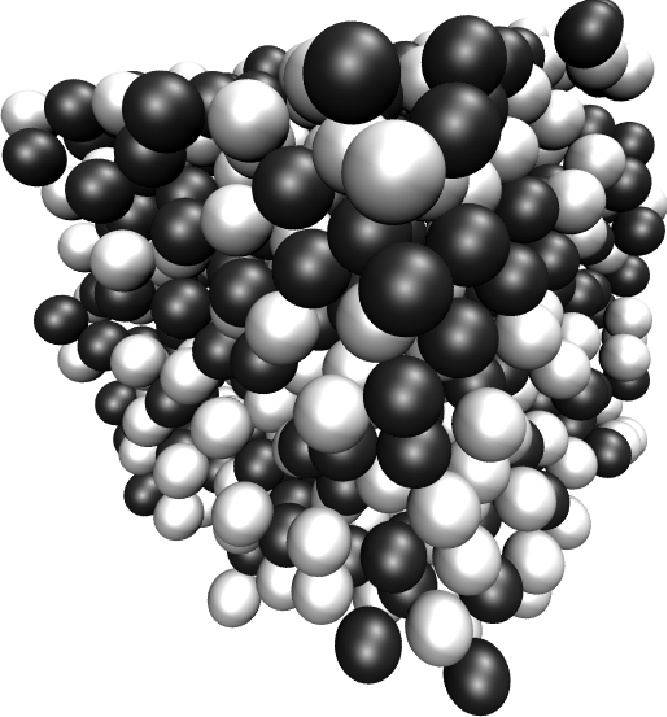
\includegraphics[width=0.4\textwidth]{figures/salt}
  \caption{VMD Snapshot of the salt system}
  \label{fig:snapshot}
\end{figure}

\section{Analysis}

For a simple analysis, we calculate the averaged radial distribution functions
$g_{++}(r)$ and $g_{+-}(r)$. We internally store particle configurations in the
integration loop by calling (after the integrate command):

\begin{lstlisting}
system.analysis.append()
\end{lstlisting}

Then, the averaged radial distribution function for all stored configurations
can be calculated using the \verb|rdf()| command from the \verb|analysis|
submodule. Add the following code after the main integration loop:

\begin{lstlisting}
rdf_bins = 100
r_min  = 0.0
r_max  = system.box_l[0]/2.0
r,rdf_00 = system.analysis.rdf(rdf_type='<rdf>', 
                            type_list_a=[0],
                            type_list_b=[0], 
                            r_min=r_min,
                            r_max=r_max, 
                            r_bins=rdf_bins)

r,rdf_01 = system.analysis.rdf(rdf_type='<rdf>', 
                            type_list_a=[0],
                            type_list_b=[1], 
                            r_min=r_min,
                            r_max=r_max, 
                            r_bins=rdf_bins)
\end{lstlisting}

The shown \verb|rdf()| commands return the radial distribution functions for
oppositely charged (0-1) and equally charged (0-0) particles for specified radii
and number of bins. In this case, we calulate the averaged rdf of the the stored
configurations, denoted by the chevrons in \verb|rdf_type='<rdf>'|. Using
\verb|rdf_type='rdf'| would simply calculate the rdf of the current particle
configuration. The results are two numpy arrays containing the $r$ and $g(r)$
values. Finally we write the data into a file:

\begin{lstlisting}
rdf_fp = open('rdf.data', 'w')
for i in range(rdf_bins):
    rdf_fp.write("%1.5e %1.5e %1.5e\n" % 
            (r[i], rdf_00[i], rdf_01[i]))
rdf_fp.close()
\end{lstlisting}

\begin{figure}[tb]
  \centering
  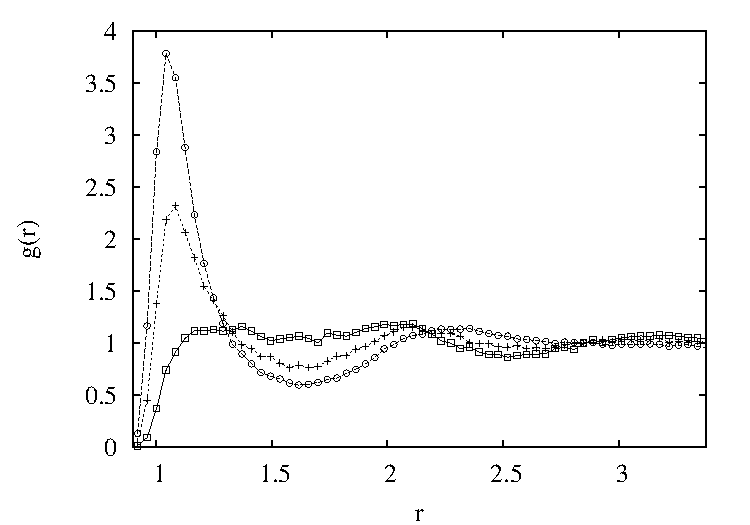
\includegraphics[width=0.7\textwidth]{figures/nacl-rdf}
  \caption{Radial distribution functions $g_{++}(r)$ between equal
    charges (rectangles) and $g_{+-}(r)$ for opposite charges
    (circles). The plus symbols denote $g(r)$ for an uncharged
    system.}
  \label{fig:rdf}
\end{figure}

Fig.~\ref{fig:rdf} shows the resulting radial distribution functions. In
addition, the distribution for a neutral system is given, which can be obtained
from our simulation script by simply not adding the P$^3$M actor to the system.
To view your own results, run \verb|gnuplot| in a Terminal window
and plot the simulation data:

\begin{lstlisting}
p 'rdf.data' u 1:2 w lp t 'g(r) ++' , '' u 1:3 w lp t 'g(r) +-'
\end{lstlisting}

%TODO
\iffalse
\section{Partially periodic boundary conditions}

\begin{figure}[h]
  \centering
  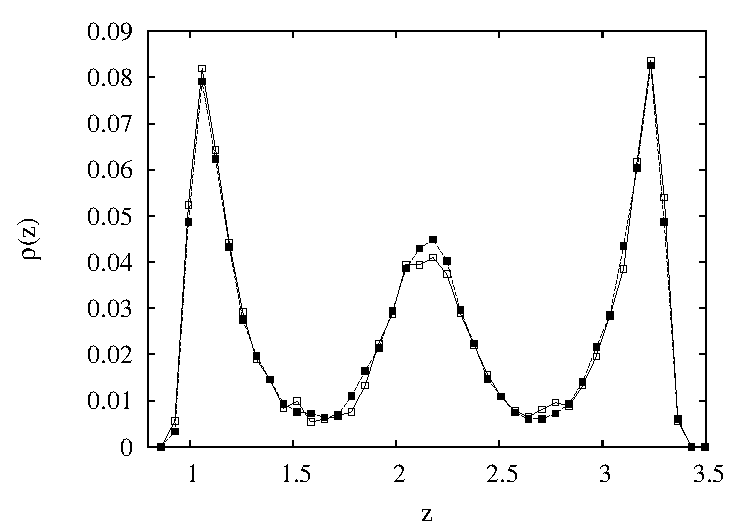
\includegraphics[width=0.7\textwidth]{figures/neutral-rho}
  \caption{Distribution of positive charges $\rho_+(z)$ (open squares)
    and of negative charges $\rho_-(z)$ (closed squares) under
    confinement along $z$.}
  \label{fig:neutralrho}
\end{figure}

One of the strengths of \es{} is the possibility to simulate charged
systems with partially periodic boundary conditions.
Before you proceed, check your \emph{myconfig.hpp} file to make
sure that the \verb|PARTIAL_PERIODIC| feature is enabled.

As an example of a system in partially-periodic boundary conditions,
we will modify our script to simulate our simple salt in a slit pore.
Remove the \verb|cellsystem|, \verb|setmd box_l| and \verb|setmd periodic| lines left
over from your previous simulation simulation script and replace them
with these lines:

\begin{lstlisting}
  set box_lxy [expr sqrt(2)*$box_l]
  set box_lz  [expr 0.5*$box_l]
  setmd box_l $box_lxy $box_lxy [expr $box_lz + 1.0]
  setmd periodic 1 1 0
  constraint wall normal 0 0  1 dist 0 type 2
  constraint wall normal 0 0 -1 dist [expr -$box_lz - 1.0] type 2
\end{lstlisting}

The final two lines add two confining walls at the top
and the bottom of the simulation box. The wall is given by its normal
vector (pointing up and downwards here), and its distance from
$(0,0,0)$. Therefore this defines one wall at $z=0$, and a second
one at $z=$\verb|box_lz|$+1$. Finally, the type of the wall is used like a
particle type to define the interaction of the walls with the particles.

The addition of $1.0$ to the slit width is due to the fact that we will
use a Lennard-Jones potential to model the wall; this means that
particles of diameter $1.0$ cannot come closer than $1.0$ to the wall. In a
way, the wall itself therefore has a thickness of $0.5$. To compensate
for this, we simply make the box bigger by 1.

We also need to choose the initial positions of our particles to match
the new box dimensions. Replace the appropriate part of your
simulation script with this random drawing of particle positions:

\begin{lstlisting}
  set posx [expr $box_lxy*[t_random]]
  set posy [expr $box_lxy*[t_random]]
  set posz [expr ($box_lz-1.0)*[t_random] + 1.0]
\end{lstlisting}

When defining the interactions, we now also need to add the
interactions between the particles and the walls, which is the same as
between the particles:

\begin{lstlisting}
  inter 0 2 lennard-jones $eps $sig $cut $shift 0
  inter 1 2 lennard-jones $eps $sig $cut $shift 0
\end{lstlisting}

For the electrostatic part, we also need to choose a different algorithm,
as P$^3$M can only handle fully periodic boundary conditions. We
choose the MMM2D method:

\begin{lstlisting}
  cellsystem layered 3
  inter coulomb 1.0 mmm2d 1e-4  
\end{lstlisting}

which replaces the \verb|inter coulomb 10.0 p3m ...| code. Note the
decreased Bjerrum length --- the confined system would take too long for
a tutorial to equilibrate with Bjerrum length 10.0. Still,
equilibrating the system is now more difficult. First, we cannot
simply ramp up all Lennard-Jones interactions anymore; otherwise,
particles will penetrate the walls and break the confinement. Second,
we need to ramp up the electrostatic interaction more carefully
now. The following code replaces the equilibration loop previously 
used. It gradually increases the Bjerrum length to the
target value of 1.0, and caps only the Lennard-Jones interactions
between the particles. The latter can be done by switching on
individual force capping, and setting a force cap radius for the
particle-particle interactions:

\begin{lstlisting}
inter forcecap individual
for {set i 1} {$i < 10} {incr i} {
    set rad [expr 1.0 - 0.5*$i/10.0]
    set lb [expr 1.0 * $i / 10.0]
    inter 0 0 lennard-jones $eps $sig $cut $shift 0 $rad
    inter 1 0 lennard-jones $eps $sig $cut $shift 0 $rad
    inter 1 1 lennard-jones $eps $sig $cut $shift 0 $rad
    inter coulomb $lb mmm2d 1e-4
    integrate $integ_steps
}
inter forcecap 0
inter coulomb 1.0 mmm2d 1e-4  
\end{lstlisting}

Finally, when writing out, we should update the set of
Tcl-variables to represent the asymmetric box, and write out
\verb|box_lxy| and \verb|box_lz| instead of just \verb|box_l|.

\subsection*{Analysis}

For a such a strongly confined system, the radially averaged
distribution function is inappropriate. Instead, it would be more
interesting to study the distribution of the particles along the slit
width. \es{}  does not provide such a function, however, we can easily
write one using the \verb|bin| command, which simply allows us 
to create a histogram based on a set of values given as a Tcl list.
Therefore, we first create the list
of z-coordinates, and then bin them:

\begin{lstlisting}
  set bins 20
  set data ""
  for {set p 0} {$p <= [setmd max_part]} {incr p} {
    lappend data [lindex [part $p pr pos] 2]
  }
  set rho [bin -linbins 0.5 [expr $box_lz + 0.5] $bins $data]
\end{lstlisting}

Here, \verb|bins| is a variable that you should set to the desired
number of bins (20 should be fine). Otherwise, this code can replace
the analyze rdf command. The \verb|bin| command can also be used to
calculate the coordinates of the bins:

\begin{lstlisting}
  bin -linbins 0.5 [expr $box_lz + 0.5] $bins -binctrwdth
\end{lstlisting}

will return a list of the centers and widths of the bins, which can be
used in analogy to \verb|rlist| in the previous analysis code. Of
course, it would be interesting to study the distribution of positive
and negative charges separately; for this, you need to duplicate the
averaging code, and use two data sets to append the z-coordinates to,
depending on the particle type:

\begin{lstlisting}
  if {[part $p pr type] == 0} {
    lappend data0 [lindex [part $p pr pos] 2]
  } {
    lappend data1 [lindex [part $p pr pos] 2]
  }
\end{lstlisting}

The resulting distribution of charges is shown in
Fig.~\ref{fig:neutralrho}. You can see a layering effect of the
confinement on the charge distributions.

\begin{figure}[h]
  \centering
  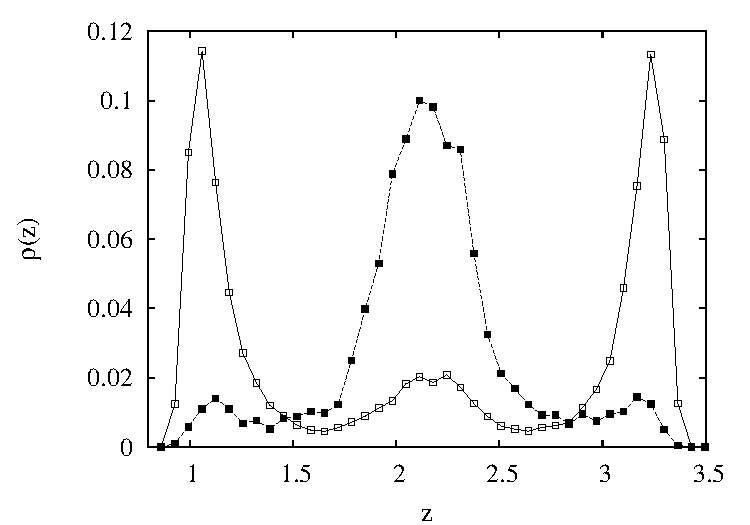
\includegraphics[width=0.7\textwidth]{figures/nonneutral-rho}
  \caption{Distribution of positive charges $\rho_+(z)$ (open squares)
    and of negative charges $\rho_-(z)$ (open squares) under
    confinement along $z$. The two confining walls are negatively
    charged, pushing away the negative charges.}
  \label{fig:nonneutralrho}
\end{figure}

\subsection*{Charging the walls}

So far, the distributions of particles of type 0 and 1 are more or
less the same, as one would expect. However, we can change this by
introducing charged walls. That is done using the
\verb|constraint plate| command:

\begin{lstlisting}
  set sigma [expr -0.25*$n_part/($box_lxy*$box_lxy)]
  constraint plate height 0 sigma $sigma
  constraint plate height [expr $box_lz + 1.0] sigma $sigma
\end{lstlisting}

Note that you need to have both the \verb|constraint plate| and the 
\verb|constraint wall| commands in your simulation script.
This adds two plates at the bottom and top of the simulation box. The
charged walls (the capacitor \emph{plates}) are necessarily
perpendicular to the z-axis, since for all electrostatics methods for
2d-periodic systems, \es{} assumes that the z-axis is the
non-periodic axis.

Note that
this adds two walls with a total charge of \verb|n_part|/2, which
would make the overall system charged. So to maintain charge
neutrality, we need to only create half of the charges (i.e. 100)
with alternating charges as before, while the rest is created
with positive charge.
For this system, you should obtain distributions as shown in
Fig.~\ref{fig:nonneutralrho}. The distribution of charges differs
strongly between the two types of charges; while the positive charges
layer at the walls, the negative charges accumulate in the center of
the system.

\fi





%\section{Accelerating the simulation using a GPU}
%TODO
\iffalse
\es{} can make use of an Nvidia graphics processing unit (GPU) for 
accelerating simulations.
Of course, we expect that results of the GPU-based implementation of
P$^3$M to be exactly identical to those of the traditional CPU
implementation. So copy the results from the previous task to a
different file name (e.g.~\verb|rdf_p3m_cpu.data|) for comparison.
Additionally, we'd like to find out exactly how much faster the GPU
implementation is. So first wrap your previous simulation script with
a time measurement, run it again and note down the execution time.
\begin{lstlisting}
	set starttime [clock seconds]
	
	# previous script code goes here
	
	set endtime [clock seconds]
	puts "Simulation took [expr $endtime-$starttime] seconds"	
\end{lstlisting}

To switch to the GPU-based implementation of 
P$^3$M, go to the line of your simulation script that contains
\verb|inter coulomb| and replace \verb|p3m| with \verb|p3m gpu|.
Then run the simulation again and note down the execution time,
which should be a lot shorter now. Plot the RDFs from both
the CPU and the GPU simulation into one graph and check whether the
results agree.
\fi

%\section{Using the MEMD algorithm}

%TODO
\iffalse
\es{} provides a variety of different electrostatics solvers. So far,
we have been introduced to P$^3$M, but in this section we will try
something new. A fairly recent addition to the family of electrostatics
solvers is the "Maxwell Equations Molecular Dynamics" (MEMD) algorithm.
To use it, two parameters have to be set: A mesh size, and a method
parameter called \verb|f_mass|, which can be estimated by a formula
given in the \es{} user guide. In this example, a good estimate for
the mesh size is 12, but this can be varied, affecting speed and
accuracy of the algorithm.

The MEMD algorithm relies on a very specific spatial distribution of
the particles across processors, and will therefore currently not work
with Verlet lists. Since those are switched on by default, they will
have to be turned off manually by adding the following line before the
\verb|setmd| commands:

\begin{lstlisting}
  cellsystem domain_decomposition -no_verlet_list
\end{lstlisting}


Besides this, you will have to replace the initialization of the
P$^3$M interaction (\verb|inter| \verb|coulomb|...) with an
appropriate one for MEMD:

\begin{lstlisting}
  set memd_mesh 12
  set f_mass [expr 100.0*pow( ([setmd time_step]*$memd_mesh/$box_l),2.0)]
  inter coulomb 10.0 memd $f_mass $memd_mesh
\end{lstlisting}


In the example script included
within the \es{} code, there is already an \verb|if|-construct 
provided and you can switch between the methods at the very top
of the script.

You can copy the results from your completed tasks so far to a different
filename (e.g.~\verb|rdf_p3m.data|) for comparison. Then, just
run the simulation and analysis again, and compare the speed and 
resulting radial distribution function of the two methods.
\fi

\end{document}
